% !TEX encoding = UTF-8 Unicode
\documentclass[convert={density=300,size=1000x700,outext=.png}]{standalone}
\usepackage{tikz}
% \usepackage[active,tightpage,psfixbb]{preview}
\usepackage{tipa}
% \PreviewEnvironment{pgfpicture}
% \setlength\PreviewBorder{2pt}

\begin{document}
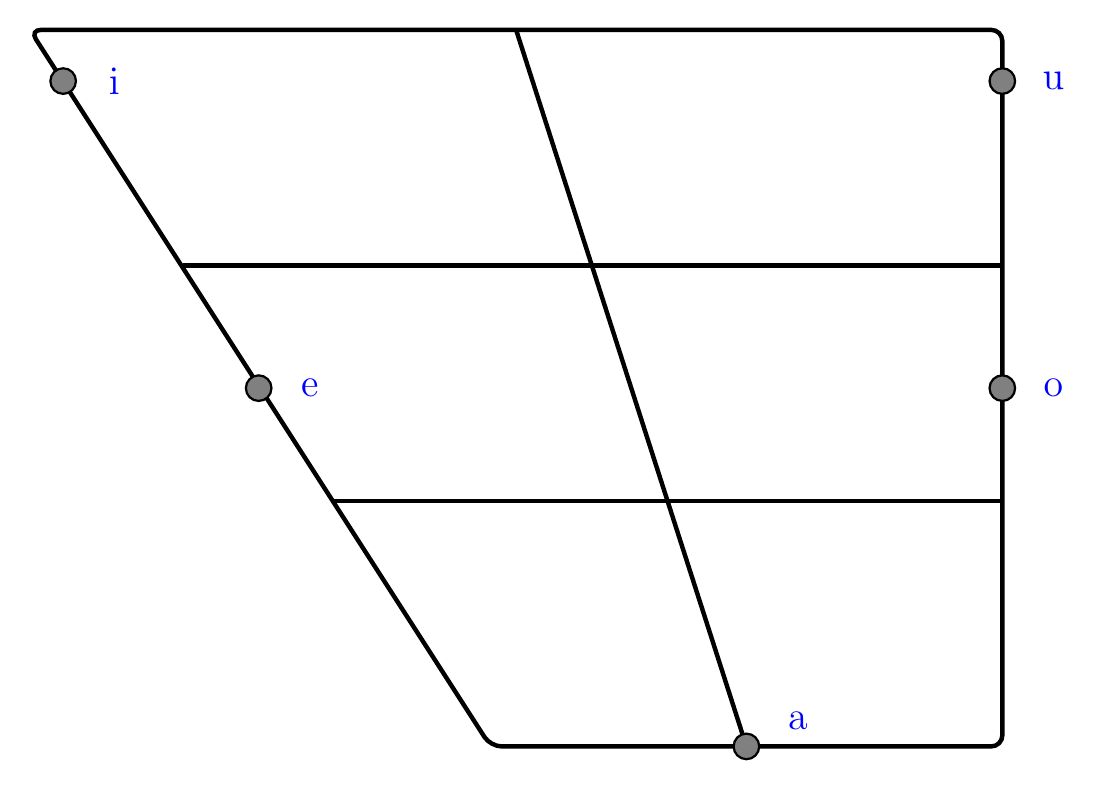
\begin{tikzpicture}[scale=.65]

% \draw[help lines] (0,0) grid (25,20);

% arrows
\draw [-, ultra thick, rounded corners] (22,16.5) -- (22,3) -- (12,3) -- (3,17) -- (22,17) -- (22,16.5);
\draw [-, ultra thick, rounded corners] (12.5,17) -- (17,3);
\draw [-, ultra thick, rounded corners] (22,12.4) -- (6,12.4);
\draw [-, ultra thick, rounded corners] (22,7.8) -- (8.9,7.8);

% vowels
\node [font=\Large,blue] at (4.65,16) {\textipa{i}};
\draw [black, thick, fill=gray] (3.65,16) circle [radius=0.25];

\node [font=\Large,blue] at (8.47,10) {\textipa{e}};
\draw [black, thick, fill=gray] (7.47,10) circle [radius=0.25];

\node [font=\Large,blue] at (18,3.5) {\textipa{a}};
\draw [black, thick, fill=gray] (17,3) circle [radius=0.25];

\node [font=\Large,blue] at (23,10) {\textipa{o}};
\draw [black, thick, fill=gray] (22,10) circle [radius=0.25];

\node [font=\Large,blue] at (23,16) {\textipa{u}};
\draw [black, thick, fill=gray] (22,16) circle [radius=0.25];

\end{tikzpicture}
\end{document}